\documentclass{article}
\usepackage{graphicx} % Required for inserting images
\usepackage[margin=1in]{geometry}
\usepackage{amsmath}
\usepackage{amsthm}
\usepackage{amssymb}
\usepackage{amsfonts}
\usepackage{enumitem}
\usepackage{verbatim}
\usepackage{xcolor}
\usepackage{soul}
\usepackage{hyperref}

\hypersetup{
    colorlinks=true,
    linkcolor=blue,
    filecolor=magenta,
    urlcolor=blue,
    pdftitle={Overleaf Example},
    }

\title{Final Project Report: Game of Life}
\author{Dante Buhl}

\DeclareMathOperator{\cond}{cond}
\DeclareMathOperator{\vecspan}{span}


\begin{document}

\newcommand{\bs}[1]{\boldsymbol{#1}}
\newcommand{\bmp}[1]{\begin{minipage}{#1\textwidth}}
\newcommand{\emp}{\end{minipage}}
\newcommand{\R}{\mathbb{R}}
%\newcommand{\Imag}{\mathbb{I}}
\newcommand{\C}{\mathbb{C}}
\newcommand{\N}{\mathcal{N}}
\newcommand{\I}{\mathrm{I}}
\newcommand{\K}{\bs{\mathrm{K}}}
\newcommand{\m}{\bs{\mu}_*}
\newcommand{\s}{\bs{\Sigma}_*}
\newcommand{\dt}{\Delta t}
\newcommand{\dr}{\Delta r}
\newcommand{\dx}{\Delta x}
\newcommand{\tr}[1]{\text{Tr}(#1)}
\newcommand{\Tr}[1]{\text{Tr}(#1)}
\newcommand{\pd}[2]{\frac{\partial #1}{\partial #2}}


\maketitle

\section*{PCAM for the Game of Life}

\begin{enumerate}[label=\alph*)]

\item[P] The problem caan be partitioned into a smallest task size of updating a
single cell in the grid. 

\item[C] The communication needed for this problem involves getting the
neighbors of a cell (or sub-grid) from other processors.

\item[A] Agglomeration involves assigning sub-grids of the original matrix to
update rather than having a processor do one cell at a time. This reduces the
communication needed by a lot. 

\item[M] Depending on it being a 1D or 2D decomposition, tasks are assigned
going downwards first and then left to right. So if its a 1D column
decomposition then taks will be assigned left to right, if its a 2D
decomposition, tasks will be assigned from the top down until the bottom of the
matrix is reached, and then left to right, repeating the veritcal process. The
algorithm will assign rows and column sizes evenly unless the partitioning size
doesn't evenly divide the grid size (in which case the end tasks are assigned an
extra row/column). 

\end{enumerate}

\section*{Instructions for Running the Code}

\begin{enumerate}[label=\alph*)]
\item There are 3 versions of this code; a serial version, a parallel 1D column
or row
decomposition (parallel\_1d), and a parallel 2D decomposition (parallel\_2d). All of the versions read in
initial states in the same way. The executable is ran with an input file called
IC or IC.dat (this is seen in the gol.slurm files in each subdirectory). In
order to compile the code just type make in each directory (in the serial
version, the makefile also runs the code). This will produce an executable
called driver.exe. Note that the makefile should include the compiler flag -cpp
and -DHB. This essentially runs the code on a version of MPI which is supported
by Hummingbird. It should also be noted that the 1D Parallel code chooses to do
a row or column decomposition based off of the boolean titled ``rowdecomp'' at
the top of that directories driver file. Then to run the code (on hummingbird) simply type sbatch
gol.slurm. This will work as long as the IC file is formatted properly. 

In order to format the IC file properly follow the guidelines here. The first
line of the IC file should be 2 integers, each in 6 digit cells. For example, if
you would like a 20 x 20 grid the first line should be, ``\_\_\_\_20\_\_\_\_20'' (latex
does spacing weirdly, the underscores should be spaces). Then the following 20
lines after that should be the matrix transposed. That is the first column of
the matrix should be the second line of the IC file. Then the second column on
line 3 and so on. Note that an active cell is labeled as 1 and an unactive cell
is labeled as 0. Also note that there should be no spaces between the cells. If
this is done correctly, then the code will read the IC file perfectly and
perform the rest of the procedure. If you would like to aadjust the number of
timesteps, go into the code and change the variable ``nt'' to whatever you would
like. 

On output, the code produces 2 files, ``gol.dat'' and ``params.dat''.
``Gol.dat'' contains the matrix values at every update printed in the same
format as the input except with spaces between the cells, and ``params.dat''
contain the gridsize and number of timesteps (plus the IC). 

In order to visualize the output, open the matlab file gol.m and run this code
within the same directory. It will read in the two output files and create a
movie. In order to adjust the speed of this movie, change the command
``movie(M,1,*)'' to whatever you would like, where the number in place of the
star will indicate the frames per second of the movie. 

That should be everything you need to know. Note that the 2D decomposition only
works on an even number of processors, a perfect square number of processors,
and a multiple of three number of processors. Information about how the
decomposition works can be found in the subroutine ``mpi\_decomp\_2d'' within the
``pgameoflife.f90'' module file. 

\end{enumerate}

\section*{Glider Test on a 20x20 grid}

\begin{enumerate}[label=\alph*)]
\item Figure 1 shows the glider test at all 4 timesteps requested. As we can see
at t = 80, the state has returned to to the initial state in the top left
corner. 
\begin{figure}
    \centering
    \bmp{1}
        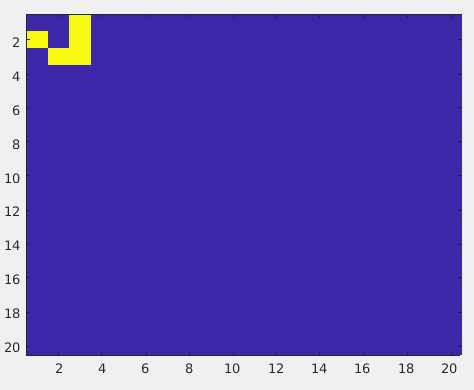
\includegraphics[width=.48\textwidth]{glidertest0.png}
        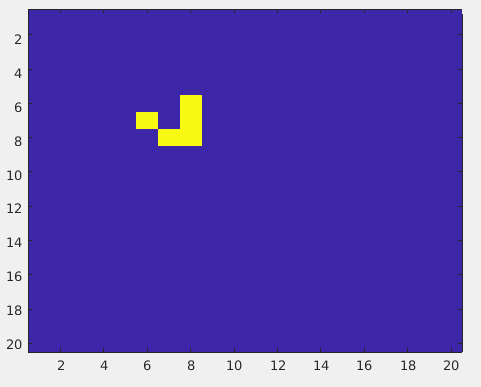
\includegraphics[width=.48\textwidth]{glidertest20.png}
    \emp

    \bmp{1}
        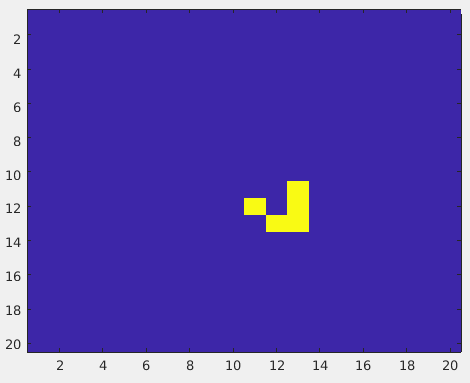
\includegraphics[width=.48\textwidth]{glidertest40.png}
        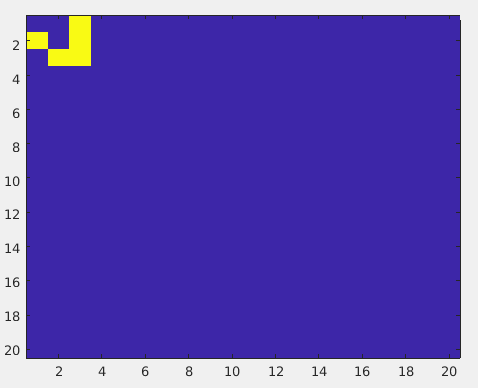
\includegraphics[width=.48\textwidth]{glidertest80.png}
    \emp
    \caption{Output from the glider IC at t = 0 (top left), t = 20 (top right),
    t = 40 (bottom left), and t = 80 (bottom right).}
\end{figure}
\end{enumerate}

\section*{Performance Model}

A performance model for the 2D case is not very hard to formulate. We look first
at the execution time, then the efficiency, and finally the isoefficiency. There
are some things to note about the communication time model for this code. Since
the IO part of the code runs in a serial manner, there is a necessary lag in the
execution time (which would be helped by using parallel IO in some regard). This
gives rise to the term quadratic in $P$ within the communication time. Each
proccessor has to wait $(P-1)$ number of subgrid communication times. Also note
that $m$ and $n$ are the sizes of the subarrays rather than the size of the global
array $M,N$. 

\begin{align*}
    T_{\text{comp}} &= t_cMN, \quad \text{no repeated computations}\\
    T_{\text{comm}} &= P(2(t_s + mt_w) + 2(t_s + nt_w) + 4(t_s + t_w)) + (P-1)P(t_s +
    mnt_w)\\
    T_{\text{IO}} &= t_IMN\\
    T_{GOL} &= \frac{T_{\text{comp}} + T_{\text{comm}}}{P} + T_{\text{IO}}\\
            &= \frac{t_cMN}{P} +
    2(t_s + mt_z) + 2(t_s + nt_w) + 4(t_s + t_w) + (P-1)(t_s+mnt_w) + t_IMN
\end{align*}
\begin{align*}
    E = \frac{t_cMN + t_IMN}{t_cMN +
    2P(t_s + mt_z) + 2P(t_s + nt_w) + 4P(t_s + t_w) + P(P-1)(t_s+mnt_w) + t_IMN}
\end{align*}
    Some remarks about the execution time and efficiency, we can see obviously
    that the execution time may increase or decrease with $P$ depending on the
    relative weight of the computation time versus the cost for the serialized
    communication in the IO. If the IO were parallelized we would see the
    execution time decrease with $P$ and there would be an lower bound of the
    communication time (not IO related). We can also see that the efficiency of
    this code decreases with $P$ rather rapidly because of the serialized
    IO structure. We can obtain the isoefficiency from this model as well and we
    see that if $P$ were to increase, we would need $M$ or $N$ to increase by
    $P^2$ in order to keep efficiency constant. Therefore the Isoefficiency is
    $O(P^2)$ which according to Nic's lecture notes, is poorly scalable. Again
    if the IO were parallelized we would see that the Isoefficiency would be
    order P, but the efficiency would still decrease with $P$, just at a slower
    rate. I didn't test the performance model, but I'm pretty sure it works like
    this. 

\end{document}
